% C14 — Traction vs counterweight trebuchet (II-11). Book: vol-2/ch-11 ¶¶ on Saianfu and the engines, Notes [24]–[37] ([@yc, 2.70]).
% Record: Yuan shi biographies of Isma'il and Ala al-Din (F-07); frame comparandum C46 (1227 Savona trestle, Annales Ianuenses).
\path (0,0) -- (11.43,0);
\node[dg-head] at (0,0.25) {Traction and counterweight stone-throwers compared};
\node[anchor=north west, inner sep=0pt] at (1.11,0.55) {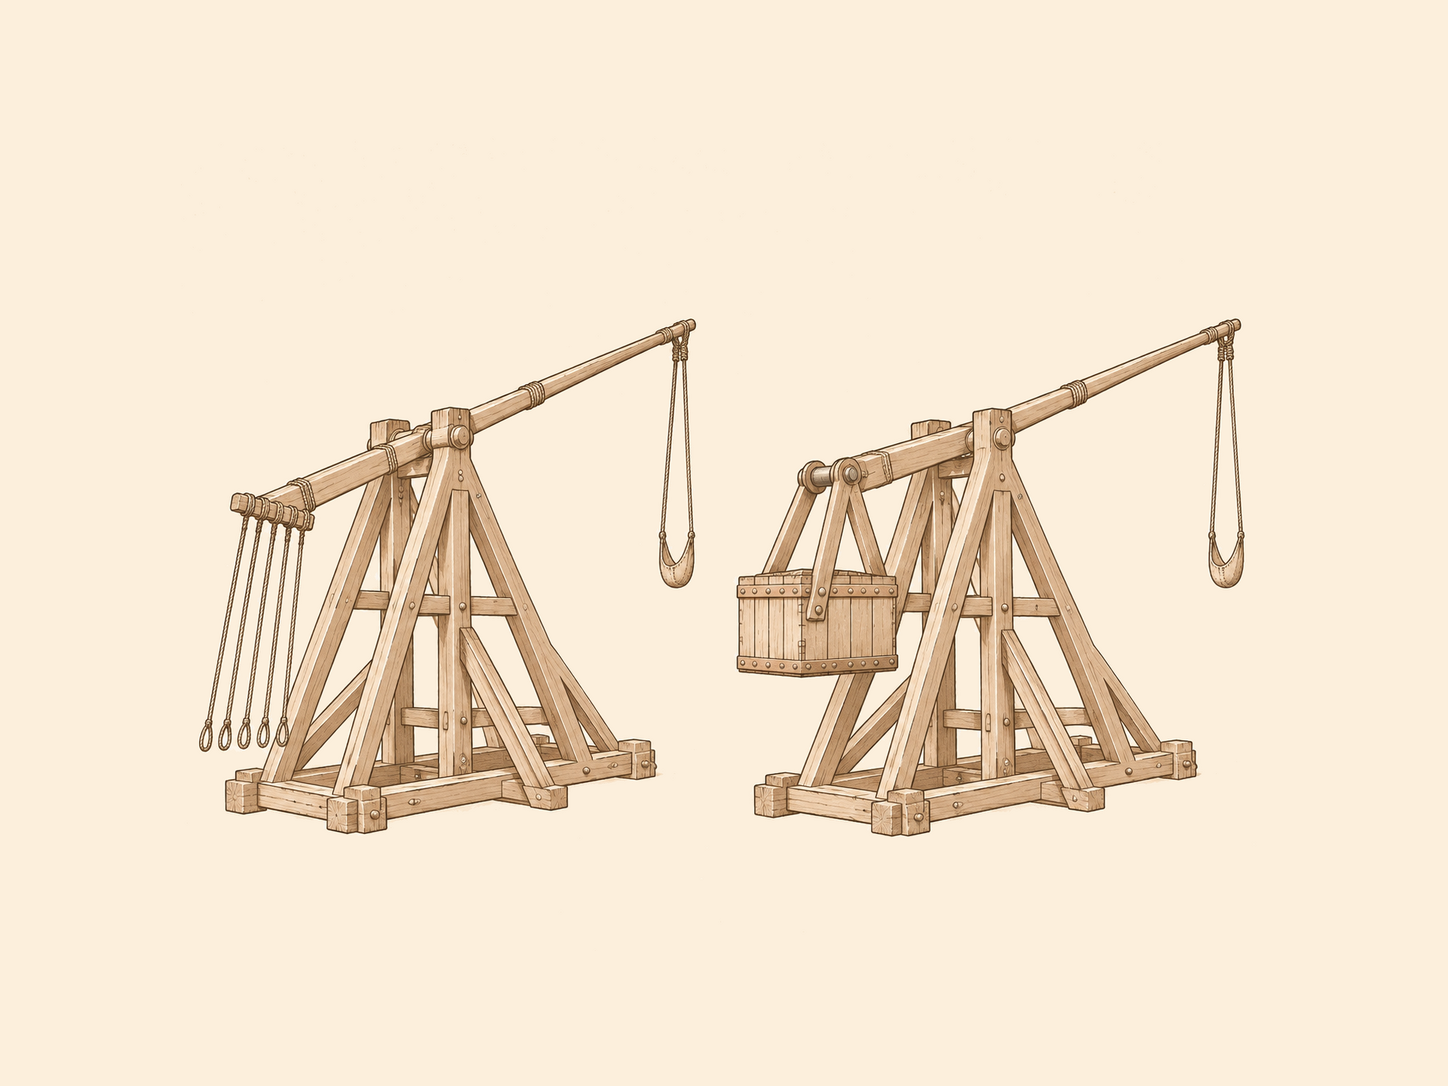
\includegraphics[width=9.20cm]{../../../manuscript/assets/plates/C14-trebuchet-comparison.png}};
% Section headers over the two machines
\node[font=\footnotesize\bfseries, text=ink, anchor=north west] at (1.40,0.95) {Traction engine (\textit{pao})};
\node[font=\scriptsize\itshape, text=inksoft, anchor=north west] at (1.40,1.32) {Used in Song and Mongol sieges};
\node[font=\footnotesize\bfseries, text=vII, anchor=north west] at (5.80,0.95) {Hinged-counterweight (\textit{Huihui pao})};
\node[font=\scriptsize\itshape, text=inksoft, anchor=north west] at (5.80,1.32) {Brought to Fancheng and Saianfu, 1272–73};
% Callouts
\draw[tl-leader] (2.60,4.40) -- (1.80,6.55);
\node[dg-text, text width=3.45cm, font=\scriptsize, anchor=north west] at (0.0,6.60) {\textbf{Pulling ropes}: a hauling crew pulls down the short arm by hand};
\draw[tl-leader] (6.20,4.25) -- (5.45,6.55);
\node[dg-text, text width=3.85cm, font=\scriptsize, anchor=north west] at (3.70,6.60) {\textbf{Pivoting ballast box}: heavy counterweight hangs on rigid arms from the short end};
\draw[tl-leader] (8.95,3.85) -- (9.15,6.55);
\node[dg-text, text width=3.55cm, font=\scriptsize, anchor=north west] at (7.80,6.60) {\textbf{Long arm \& sling}: Polo gives 300-lb stones; Yule's Chinese notice $\sim$166 lb};
\node[dg-note, text width=11.2cm] at (0,7.75) {Schematic comparison of operating principles. Neither the \textit{Yuan shi} nor Polo records the exact frame geometry of the 1272–73 engines built by Alawating and Ysemain.};
